\cleardoublepage

\section{开题报告}

\subsection{问题提出的背景}

\subsubsection{背景介绍}

引用文献 \upcite{article1} \upcite{article2}
\subsubsection{本研究的意义和目的}
多空一行表示分段

这是一个公式
\begin{equation}
	\label{eq:eqlabel}
E = mc^2
\end{equation}
引用公式 \eqref{eq:eqlabel}
\subsection{论文的主要内容和技术路线}

\subsubsection{主要研究内容}

插入一张图片
\begin{figure}
    \centering
	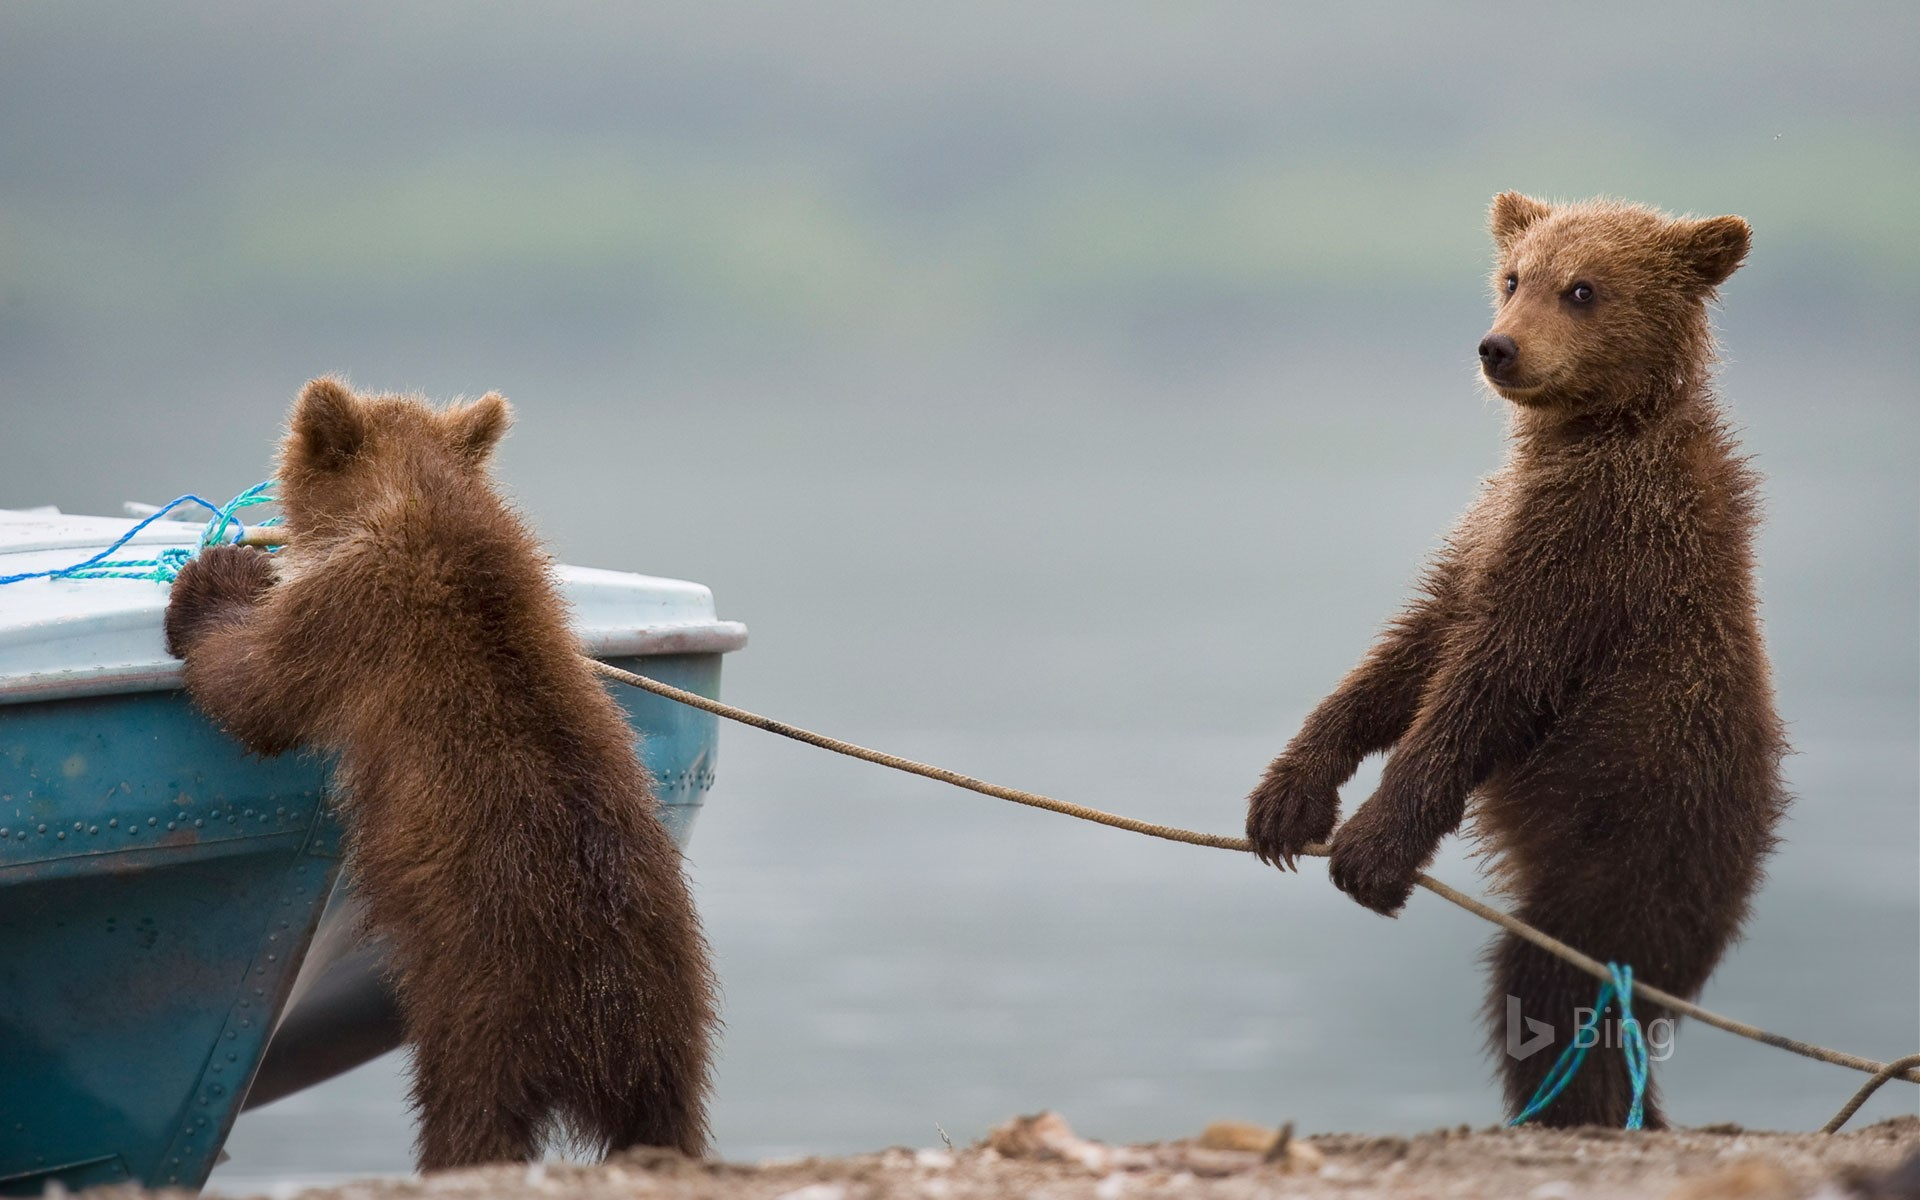
\includegraphics[width=0.5\textwidth]{images/BingWallpaper-2019-04-01.jpg}
	\caption{figure one}
    \label{fig:figlabel}
\end{figure}

引用图 \ref{fig:figlabel}

引用文献1 \upcite{article1} 文献2\upcite{article2}
引用多篇文献 \upcite{article1,article2}
\subsubsection{技术路线}

\subsubsection{可行性分析}

\subsection{研究计划进度安排及预期目标}

\subsubsection{进度安排}


\subsubsection{预期目标}


% 参考文献
\clearpage
\bibliographystyle{gbt7714-numerical}
\phantomsection
\subsection{参考文献}
{\normalfont\CJKfamily{Songti}\zihao{5}\setlength{\baselineskip}{14pt}
\renewcommand{\refname}{\vspace{-\baselineskip}}
\bibliography{reference/references}}